\section{Structural Elements of the Framework}\label{sec:tech-strategy}

This section provides a detailed discussion on the main components of the framework. It also includes an analysis of the probes, their use cases, and their benefits. After that, it discusses what UDS is and, finally, the visualizer.~\autoref{fig_vision} shows the conceptual working of the framework's three main components: Probes, UDS, and Visualizer.

\begin{figure}[H]
    \centering
    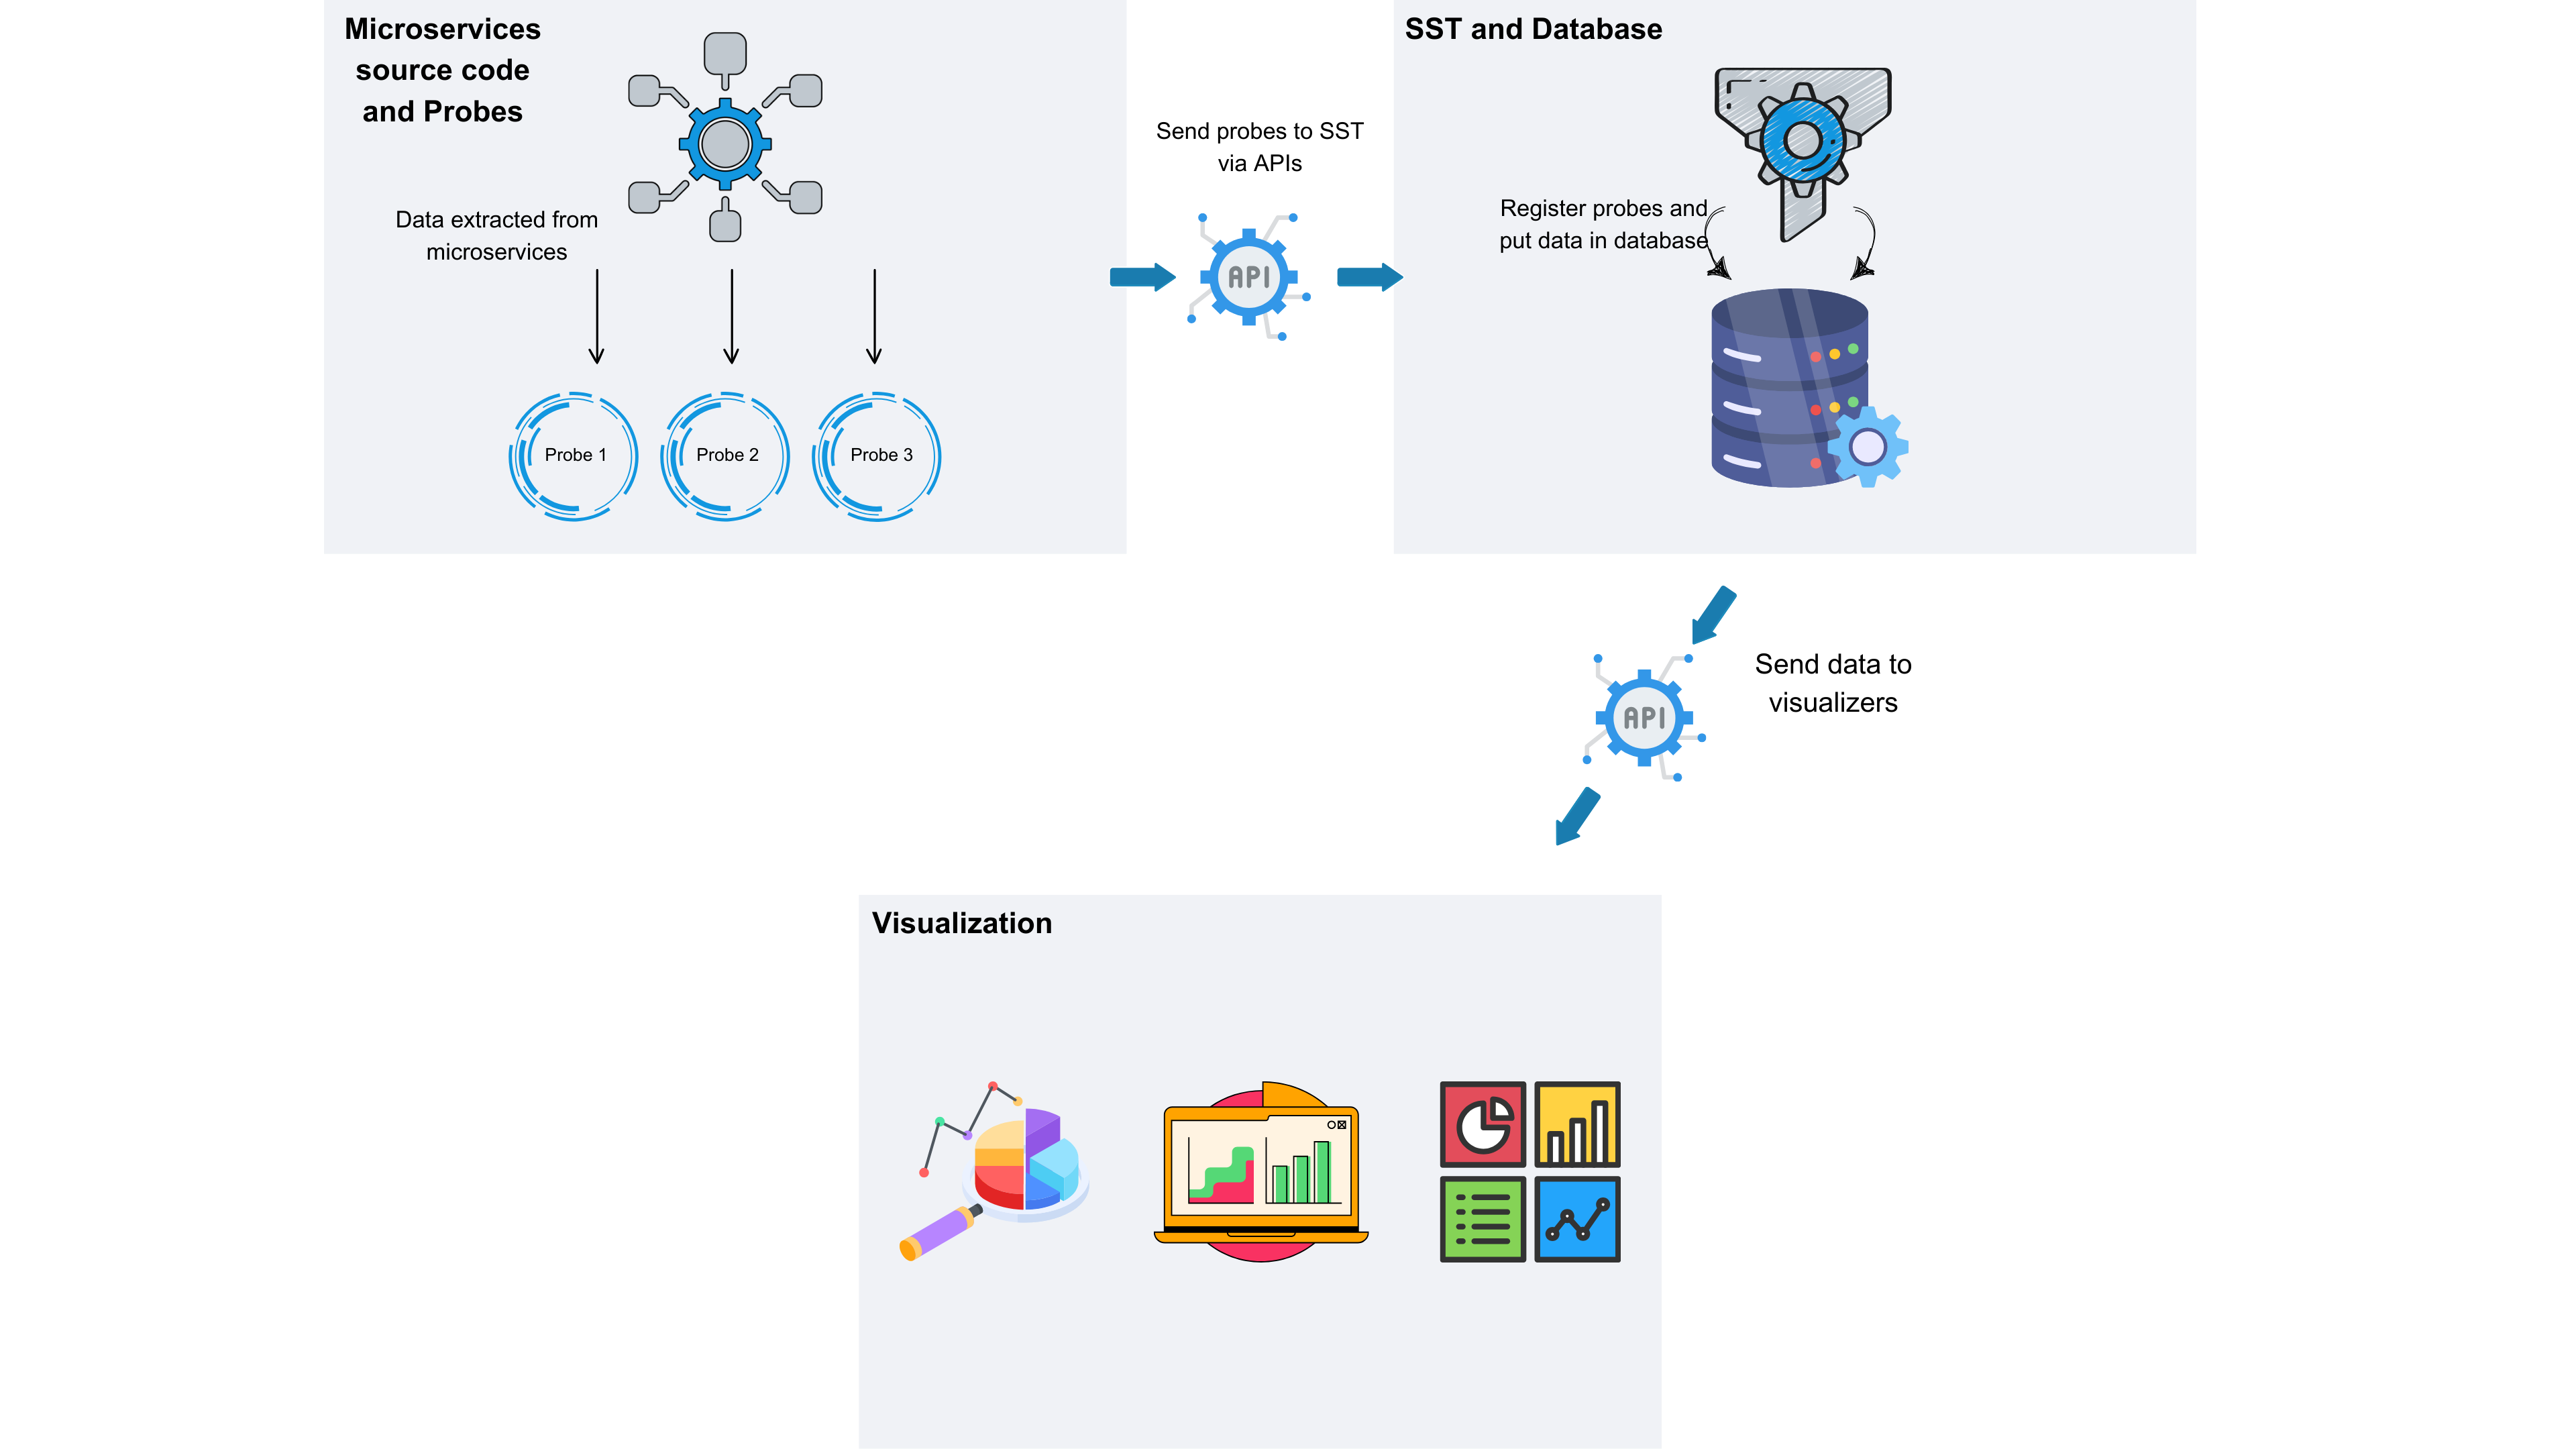
\includegraphics[width=1\textwidth]{figures/vision.png}
    \caption[Framework working]{Working of Probes, UDS and Visualizer}
	\label{fig_vision}
\end{figure}

\subsection{Probes: Extractors}\label{sec:component-probes}

The first component of the framework consists of \textbf{probes}. Probes represent distinct informational artifacts that are systematically extracted from software systems to provide insights and actionable data. In the context of this report, we have several use cases to extract specific pieces of information that are detailed in the below sections. These probes will help prove the framework credibility and serve as the foundational elements for gathering critical data points that enable analysis and decision-making. 

Looking forward, this concept can be expanded to more complex and targeted informational needs. By refining the scope and nature of the probes, we can tailor the probes according to our needs and to capture more refined data, addressing evolving requirements and insights that drive meaningful outcomes. This flexibility ensures that as the systems grow or change, the framework remains relevant and capable of producing deeper, more impactful information.

\subsection{Unified Data Source (UDS)}\label{sec:component-sst}

When data is being extracted from diverse sources, there are high chances of it becoming inconsistent and stale. In ~\autoref{sec:vision}, the visualizer component is mentioned which runs desired analysis on the data and provide visual updates. So, if analysis is to be done on the input data, it needs to be accessible, credible, reliable, and consistent.

Maintaining data quality is crucial for accurate insights and decision-making. Unified sources ensure that the input data remains clean and updated, regardless of its origin. Properly validated and processed data serves as the foundation for meaningful analysis and visualization.

A scalable and extensible approach exists for software analysis and visualization in which data from diverse source is integrated into a unified source. A \textit{unified data source} provides a single access point for querying diverse data, eliminating the need to manage multiple disconnected sources~\citep{MullerUdsforSA2018}.

There are multiple UDS tools available, but the tool used in this framework is the one developed by my colleague, Stepan Bryantsev, a member of the McMaster university McSCert team\footnote{\url{https://www.mcscert.ca/}}. This tool, called \textit{single source of truth (SST)}, consumes data from the probes, creates relationship mappings, and stores it in graphical form using the Neo4J database\footnote{\url{https://neo4j.com/}}. It is working as a data warehouse that takes all the information from diverse sources and process it. A detailed discussion on the working of the single source of truth can be found in~\autoref{chap:implementation_report} and the validation of its output will be discussed in~\autoref{chap:scenario_validations}.

\subsection{Integration and Output}

The probes will extract the required data from the microservices and feed them to the SST for further processing. The SST will generate output which will be used by the visualizer for further analysis and visualization.

\subsection{Data Management}

The output of the SST will be stored in a separate database to maintain and preserve historical records. It will help ensure that the data is structured, organized, and easily retrievable from a centralized repository. By consolidating the data into a single repository, it not only simplifies access but also certify a consistent format. 

Storing the data in a database enhances its integrity by eliminating inconsistencies and reducing complexities, such as duplicate entries. This structure allows analysts or analysis tools to focus on extracting meaningful insights without the additional work of cleaning or reorganizing raw data.

Additionally, a dedicated database supports scalability, meaning it can accommodate larger datasets as the system evolves. It also offers improved data management capabilities, such as access controls and backup solutions.

\subsection{Visualizer}\label{sec:component-visualizer}

After software analysis is completed with the help of probes and SST, we can use some visualizer tools in order to produce useful information gathered from the software system. There are diverse range of software visualization and analysis tools available in the market, with each of them having their own strengths and weaknesses. Sarita Bassil and Rudolf K. Keller covers more than 40 tools for software visualization with each having their own advantages~\citep{SWVizTools2001}. For example, Rigi is used for understanding legacy system, GraphViz is popular for graph-based visualizations and daVinci offers dynamic graph layouts.

Following are some of the important tools offered by AWS and Azure for visualization.
\begin{itemize}[label=$\bullet$]
	\item \textbf{Amazon QuickSight}: A Business Intelligence (BI) service that enables users to visualize data through dashboards, interactive graphs, and analytics. It connects to various data sources, including software systems, databases, and AWS services and perform real-time data analysis. Read more about this from~\citep{AWSQuickSight2025}. 
	\item \textbf{Amazon X-Ray}: A service for analyzing and debugging applications. It collects data about requests to your applications, including errors and performance bottlenecks. Visualizes the application architecture in a service map for easy identification of issues. Read more about this from~\citep{AWSXRay2025}.
	\item \textbf{Azure Monitor}: Azure monitor collects, analyzes, and visualizes telemetry data from azure and on-premise environments to monitor application performance and detect issues. Key features are logs and metrics collection for in-depth analysis, provides alerts and insights to troubleshoot issues in real-time~\citep{AzureMonitor2025}.
	
	\begin{figure}[H]
		\centering
		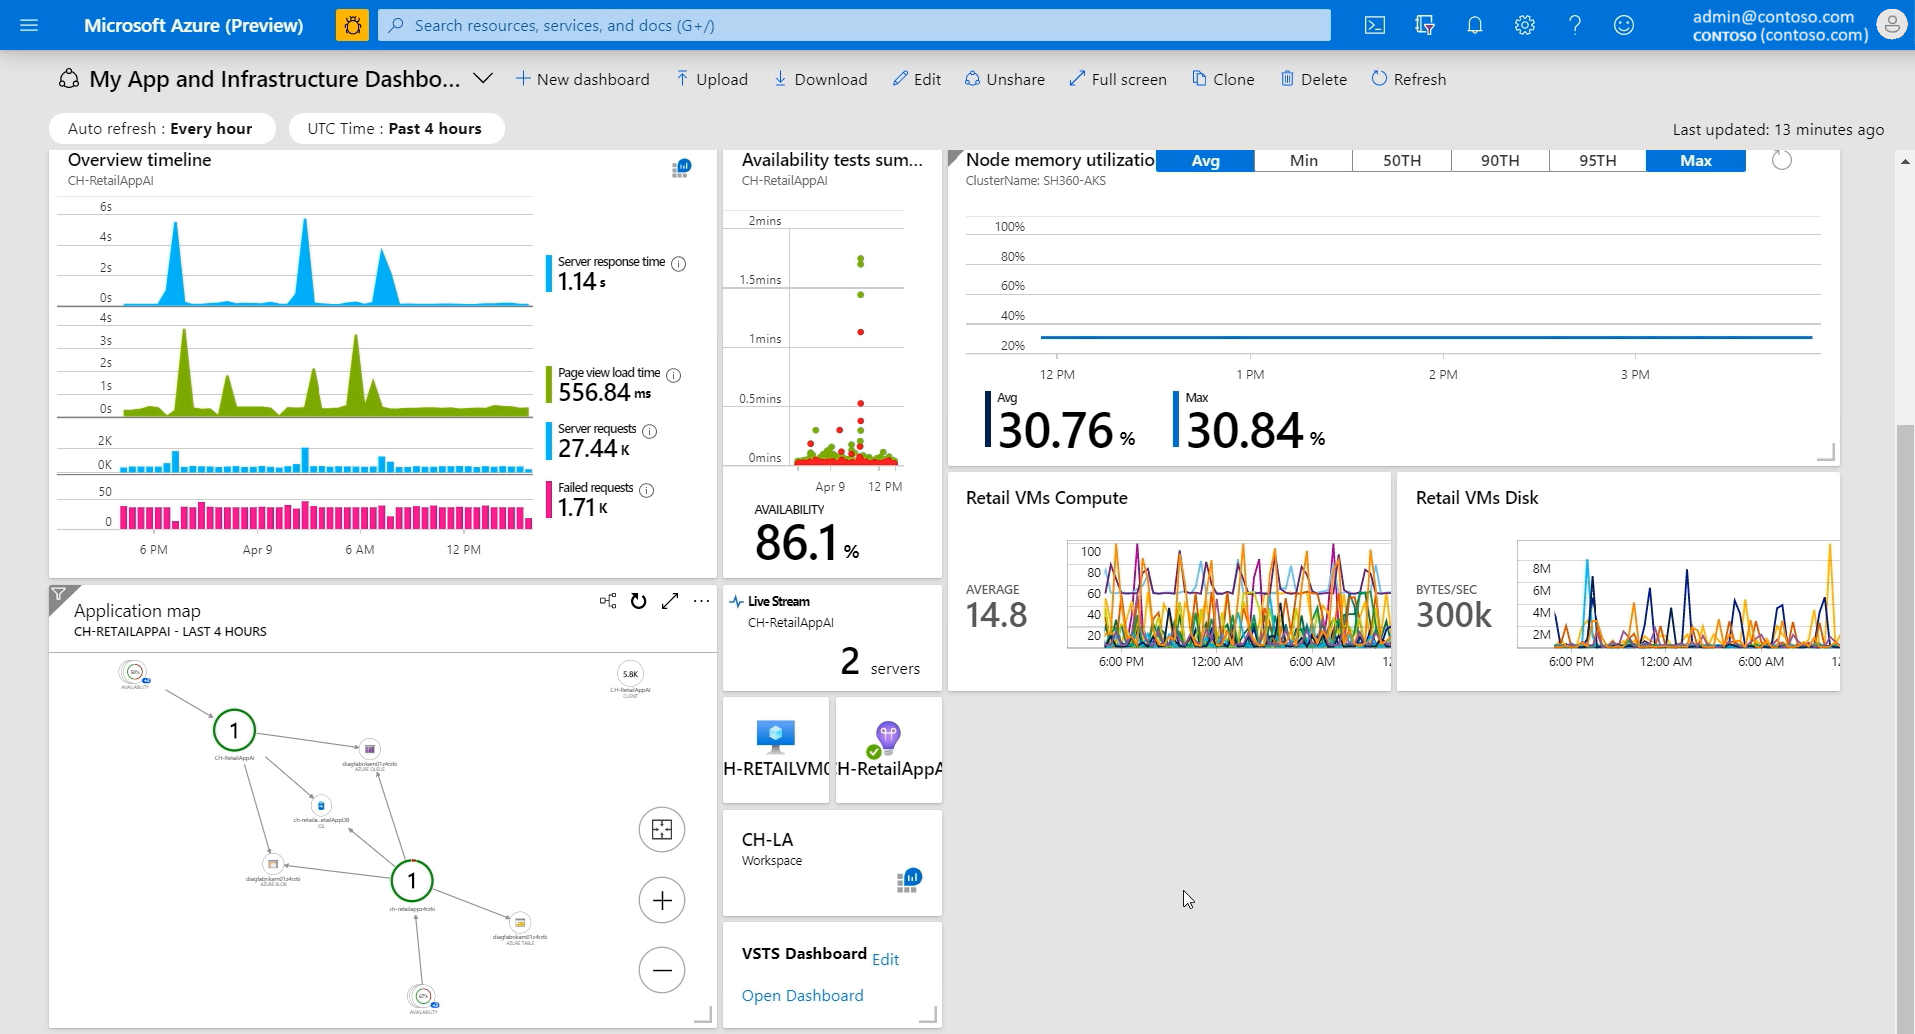
\includegraphics[width=0.9\textwidth]{figures/azure_monitor_dashboard.png}
		\caption[Azure Monitor]{Dashboard of Azure monitor (adapted from~\cite{AzureMonitorBestPractices2025})}
		\label{fig_azure_monitor}
	\end{figure}

\end{itemize}

In our report, once the probes and SST are integrated, the processed data from SST will be used for the visualization of data produced by the above mentioned probes. 